\newpage
\section{Accountancy}
\label{sec:accountancy}

The accountancy package contains functionality pertaining to book keeping.
As in other packages, interfaces are used to separate between behaviour and implementation.
\code{AccountancyEntry} is a representation of an accounting entry.
\code{Accountancy} aggregates \code{AccountancyEntry}s.
By implementing and subclassing \code{AccountancyEntry} the notion of different accounts, as known from double-entry bookkepping, can be realised.
Every \code{AccountancyEntry} is uniquely identified by an \code{AccountancyEntryIdentifier}.
\\

\code{PersistentAccountancyEntry} implements \code{AccountancyEntry} and serves as persistence entity, while \code{PersistentAccountancy} implements \code{Accountancy} and provides opaque access to the JPA layer.
\code{AccountancyEntryIdentifier} is used as primary key attribute, when persisting entities to the database.
\\

As can be seen in Figure \ref{accountancy_overview}, \code{PersistentAccountancyEntry} is sub classed to create a second ``account'' used to store payment information, namely \code{ProductPaymentEntry}.
To access entries of only one type, thus belonging to one ``account'', \code{get()} and \code{find()} methods in \code{Accountancy} have a type parameter.

Payment information also includes a user identifier referencing the buyer, an order identifier referring to the \code{Order} which was payed, and a \code{PaymentMethod} describing the money transfer.
The inheritance hierarchy of \code{PaymentMethod} is depicted in Figure \ref{payment_overview}.
\begin{figure}
	\centering
  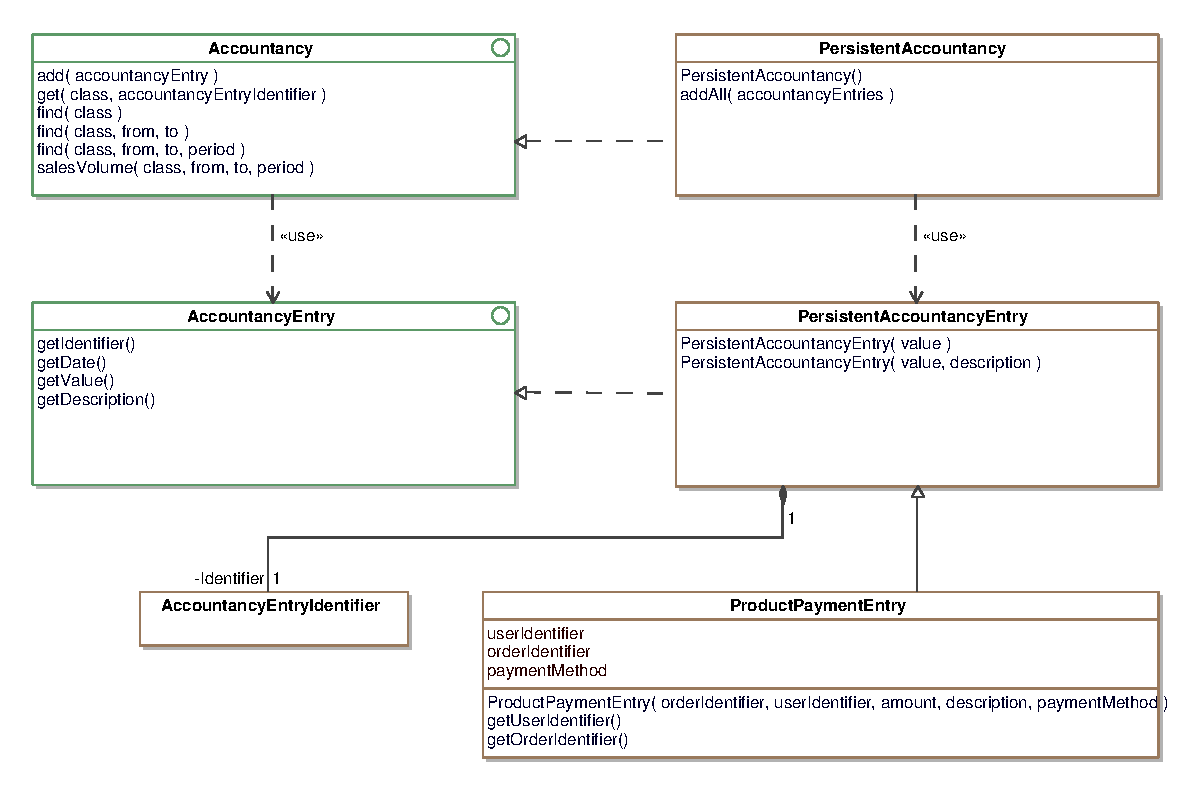
\includegraphics[width=1.0\textwidth]{images/Accountancy_Overview.eps}
	\label{accountancy_overview}
	\caption{Accountancy - Class Overview}
\end{figure}

\begin{figure}
\centering
  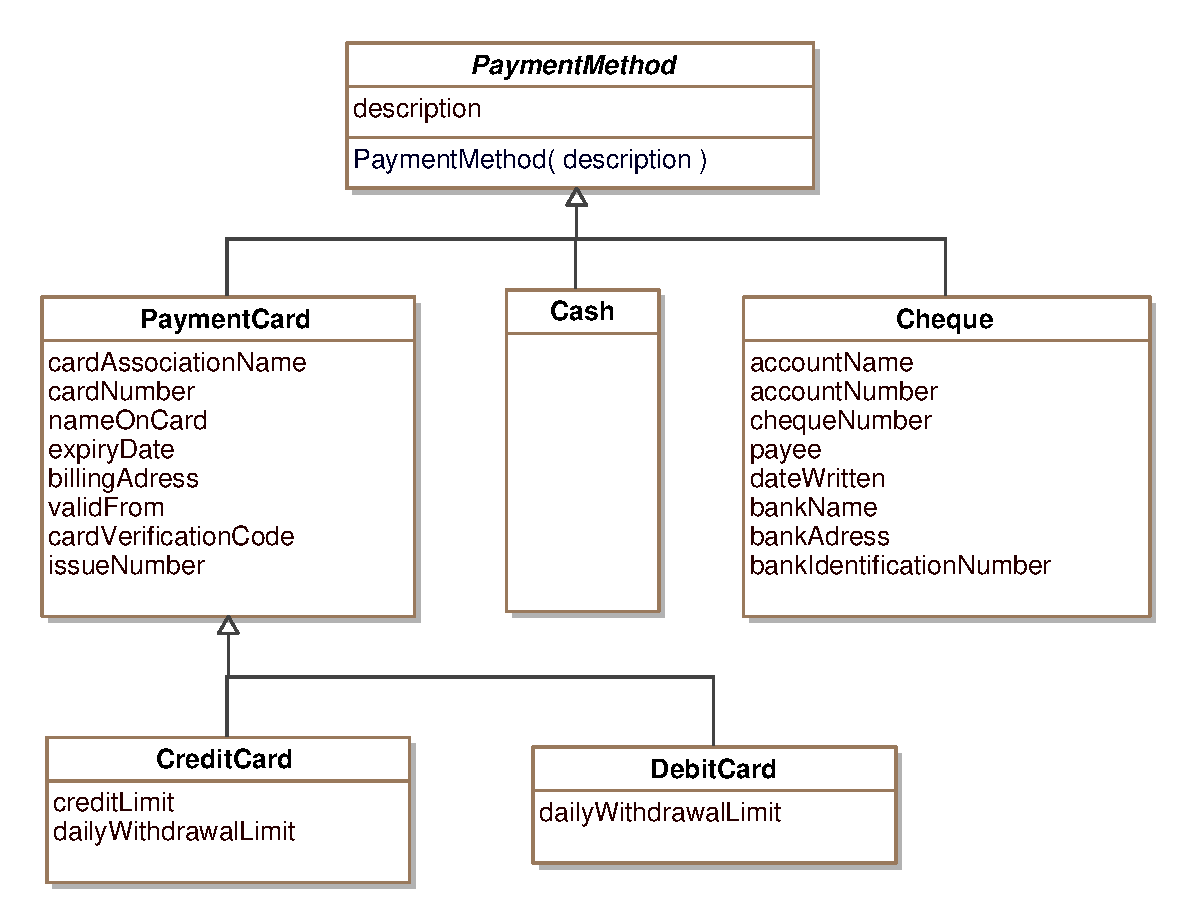
\includegraphics[width=1.0\textwidth]{images/Payment_Overview.eps}
	\label{payment_overview}
	\caption{Payment - Class Overview}
\end{figure}
